\chapter{Analysis Techniques}\label{ch:analysis}
This chapter provides some useful techniques to analyse FD schemes. Techniques to analyse PDEs also exist, but the focus here is of a practical nature and will especially revolve around the discrete schemes. This chapter can be seen as a `tutorial' on how to use these techniques. 
Starting off with some necessary theory on matrices in a FDTD context and other mathematical tools, this chapter continues to introduce 
\begin{itemize}
    \item \textit{Frequency domain analysis}, which can be used to determine stability conditions of (linear and time-invariant) FD schemes,
    \item \textit{Energy analysis}, which can both be used to debug implementations of FD schemes, as well as determine stability conditions in a more general fashion, and
    \item \textit{Modal analysis} which can be used to determine the modal frequencies (and damping per mode) that a FD scheme exhibits.
\end{itemize}

\section{Matrices in a FDTD context}\label{sec:matricesFDTD}
For several purposes, such as implementation in \texttt{MATLAB} and several analysis techniques described shortly, it is useful to write a FD scheme in \textit{matrix form}.\footnote{Appendix \ref{app:matrices} provides some basic knowledge on matrices and linear algebra for those unfamiliar with this.} Matrix multiplication when working with FDTD methods usually involves multiplying a square matrix (with equal rows and columns) onto a column vector. Consider a $(N+1)\times (N+1)$ square matrix $\A$ and a $(N+1) \times 1$ column vector $\u$. Multiplying these results in a $(N+1) \times 1$ column vector $\w$:
\begin{equation}
    \A\u = \w.
\end{equation}
Expanding this operation results in
\begin{equation}
    \underbrace{\begin{bmatrix}
        a_{00} & a_{01} & \hdots & a_{0N}\\
        a_{10} & a_{11} & \hdots & a_{2N}\\
        \vdots & \vdots & &\vdots\\
        a_{N0} & a_{N1} & \hdots & a_{NN}
    \end{bmatrix}}_{\A}
    \underbrace{\begin{bmatrix}
        u_0\\
        u_1\\
        \vdots\\
        u_N
    \end{bmatrix}}_{\u} = 
    \underbrace{\begin{bmatrix}
        a_{00}u_0 + a_{01}u_1 + \hdots + a_{0N}u_N\\
        a_{10}u_0 + a_{11}u_1 + \hdots + a_{1N}u_N\\
        \vdots\\
        a_{N0}u_0 + a_{N1}u_1 + \hdots + a_{NN}u_N
    \end{bmatrix}}_{\w}
\end{equation}
where the indexing of the matrix elements starts at $0$ rather than $1$ here, as it relates better to operations used in a FDTD context.

\subsection{FD operators in matrix form}
FD operators approximating spatial derivatives and averages introduced in Section \ref{sec:FDoperators} can be written in matrix form and applied to a column vector $\u^n$ containing the state of the system at time index $n$. These matrices are square and their sizes depend on the number of grid points the system is described for and on the boundary conditions. Not assuming a specific size for now, the FD operators in \eqref{eq:discFirstSpace} can be written in matrix form according to
% \setstackgap{L}{1.1\baselineskip}
% \fixTABwidth{T}
\setstackgap{L}{14pt}
\setstacktabbedgap{4pt}
\def\lrgap{\kern3pt}
\fixTABwidth{T}

\def\xbracketMatrixstack#1{\left[\lrgap\tabbedCenterstack{#1}\lrgap\right]}

\begin{equation*}
    \mathbf{D}_{x+} = \frac{1}{h}\xbracketMatrixstack{
        \ddots &\ddots & & & \mathbf{0}&\\
         & -1 & 1 & & & \\
        & & -1 & 1 & & \\
        & & & -1 & 1 & \\
        & & & & -1 & \ddots\\
        &\mathbf{0} & & & & \ddots
    }\qquad \mathbf{D}_{x-} = \frac{1}{h}\xbracketMatrixstack{
        \ddots & & & & \mathbf{0}&\\
        \ddots & 1 & & & & \\
        & -1 & 1 & & & \\
        & & -1 & 1 & & \\
        & & & -1 & 1 & \\
        &\mathbf{0} & & & \ddots & \ddots
    }
\end{equation*}

\begin{equation*}
    \mathbf{D}_{x\cdot} = \frac{1}{2h}\xbracketMatrixstack{
        \ddots &\ddots & & & \mathbf{0}&\\
        \ddots & 0 & 1 & & & \\
        & -1 & 0 & 1 & & \\
        & & -1 & 0 & 1 & \\
        & & & -1 & 0 & \ddots \\
        &\mathbf{0} & & & \ddots & \ddots
    }
\end{equation*}
% \begin{gather*}
%     \mathbf{D}_{x+} = \frac{1}{h}
%     \begin{bmatrix}
%         \ddots &\ddots & & & \mathbf{0}&\\
%          & -1 & 1 & & & \\
%         & & -1 & 1 & & \\
%         & & & -1 & 1 & \\
%         & & & & -1 & \ddots\\
%         &\mathbf{0} & & & & \ddots \\
%     \end{bmatrix}
%     \quad
%     \mathbf{D}_{x-} = \frac{1}{h}\begin{bmatrix}
%         \ddots & & & & \mathbf{0}&\\
%         \ddots & 1 & & & & \\
%         & -1 & 1 & & & \\
%         & & -1 & 1 & & \\
%         & & & -1 & 1 & \\
%         &\mathbf{0} & & & \ddots & \ddots \\
%     \end{bmatrix}\\
%     \\
%     \mathbf{D}_{x\cdot} = \frac{1}{2h}\begin{bmatrix}
%         \ddots &\ddots & & & \mathbf{0}&\\
%         \ddots & 0 & 1 & & & \\
%         & -1 & 0 & 1 & & \\
%         & & -1 & 0 & 1 & \\
%         & & & -1 & 0 & \ddots \\
%         &\mathbf{0} & & & \ddots & \ddots \\
%     \end{bmatrix}\\
% \end{gather*}
%
where the diagonal dots denote that the values on the respective diagonals continue until the top-left and bottom-right corners of the matrix.\todo{is this how you explain it?} The $\boldsymbol{0}$s indicate that the rest of the values in the matrix are zeros.

Averaging operators $\mxp$, $\mxm$ and $\mxd$ are defined in a similar way:

\begin{equation*}
    \mathbf{M}_{x+} = \frac{1}{2}\xbracketMatrixstack{
        \ddots &\ddots & & & \mathbf{0}&\\
         & 1 & 1 & & & \\
        & & 1 & 1 & & \\
        & & & 1 & 1 & \\
        & & & & 1 & \ddots\\
        &\mathbf{0} & & & & \ddots
    }
    \qquad
    \mathbf{M}_{x-} = \frac{1}{2}\xbracketMatrixstack{
        \ddots & & & & \mathbf{0}&\\
        \ddots & 1 & & & & \\
        & 1 & 1 & & & \\
        & & 1 & 1 & & \\
        & & & 1 & 1 & \\
        &\mathbf{0} & & & \ddots & \ddots
    }
\end{equation*}

\begin{equation*}    
    \mathbf{M}_{x\cdot} = \frac{1}{2}\xbracketMatrixstack{
        \ddots &\ddots & & & \mathbf{0}&\\
        \ddots & 0 & 1 & & & \\
        & 1 & 0 & 1 & & \\
        & & 1 & 0 & 1 & \\
        & & & 1 & 0 & \ddots \\
        &\mathbf{0} & & & \ddots & \ddots
    }
\end{equation*}

It is important to notice that only spatial operators are written in this matrix form and then applied to state vectors at different time steps ($\u^{n+1}$, $\u^n$ and $\u^{n-1}$). 

Finally, the identity matrix is a matrix with only $1$s on the diagonal and $0$s elsewhere:
\begin{equation*}
    \I = \xbracketMatrixstack{
        \ddots & & & & \mathbf{0}&\\
         & 1 & & & & \\
        & & 1 & & & \\
        & & & 1 & & \\
        & & & & 1 & \\
        &\mathbf{0} & & &  & \ddots
    },
\end{equation*}
and has the following special property
\begin{equation*}
    \I\A = \A\I = \A.
\end{equation*}

\subsection{Schemes and update equations in matrix form}\label{sec:matrixForm}
With the spatial operators in matrix form presented above, the FD scheme of the 1D wave equation in Eq. \eqref{eq:1DwaveFDS} can be written in matrix form.

If the Dirichlet boundary conditions in \eqref{eq:discreteDirichlet} are used, the end points of the system do not have to be included in the calculation. The values of the grid function $\uln$ for $l\in \{1, \hdots, N-1\}$ can then be stored in a column vector according to $\u^n = [u_1^n, \hdots, u_{N-1}^n]^T$. Furthermore, $(N-1) \times (N-1)$ matrix $\Dxx$ is defined as
\begin{equation}\label{eq:DxxDef}
    \Dxx = \frac{1}{h^2}\xbracketMatrixstack{
        -2 & 1 & & &\mathbf{0}\\
        1 & -2 & 1 & & \\
        & \ddots & \ddots & \ddots & \\
        & & 1 & -2 & 1 \\
        \mathbf{0}& & & 1 & -2 
    }.
\end{equation}
If instead, Neumann boundary conditions in Eq. \eqref{eq:discreteDirichlet} are used, the values of $\uln$ for the full range $l\in \{0, \hdots, N\}$ need to be stored as $\u^n=[u_0^n, \hdots, u_N^n]^T$ and the $(N+1) \times (N+1)$ matrix $\Dxx$ will be 
\begin{equation}\label{eq:DxxDefNeumann}
    \Dxx = \frac{1}{h^2}
    \xbracketMatrixstack{
        -2 & 2 & & &\mathbf{0}\\
        1 & -2 & 1 & & \\
        & \ddots & \ddots & \ddots & \\
        & & 1 & -2 & 1 \\
        \mathbf{0}& & & 2 & -2 
    },
\end{equation}
where the $2$s in the top and bottom row correspond to the multiplication by $2$ with $u_1^n$ and $u_{N-1}^n$ in update equations \eqref{eq:1DWaveLeftBound} and \eqref{eq:1DWaveRightBound} respectively.

Regardless of the boundary conditions, the FD scheme in \eqref{eq:1DwaveFDS} can be written in matrix form as
\begin{equation}\label{eq:1DwaveMatrix}
    \frac{1}{k^2}\left(\u^{n+1} - 2 \u + \u^{n-1}\right) = c^2 \Dxx \u^n,
\end{equation}
and rewritten to a matrix form of the update equation analogous to Eq. \eqref{eq:1DwaveUpdate}
\begin{equation}
    \u^{n+1} = (2\I + c^2k^2 \Dxx )\u^n - \u^{n-1}.
\end{equation}
The identity matrix is necessary here for correct matrix addition.

\section{Mathematical tools and product identities}
Some useful mathematical tools used for the energy analysis techniques presented in Section \ref{sec:energyAnalysis} will be shown here. The tools shown here can be applied to 1D systems. These will be extended to 2D systems in Chapter \ref{ch:2Dsyst}. Unless denoted otherwise, the notation and theory will follow \cite{theBible}.

\subsection{Inner product}\label{sec:innerProduct}
For two functions $f = f(x,t)$ and $g = g(x,t)$ defined for $x\in\D$ where $\mathcal{D} = [0,L]$, their $l_2$ inner product and $l_2$ norm are defined as
\begin{equation}\label{eq:contInnerProd}
    \langle f, g\rangle_\D = \int_\D fg dx \quad \text{and} \quad \lVert f \rVert_\D = \sqrt{\langle f, f \rangle_\D}.
\end{equation}
These functions do not have to be time-dependent (i.e., they can also simply be $f(x)$ and $g(x)$), but as all functions used in this work are in fact time-dependent, this is left for coherence. It is also important to note that these functions do not have to be `isolated' state variables per se (such as $u(x,t)$ used in the previous chapter), but could also be state variables with a derivative applied to it (such as $\pt u(x,t)$). 

The discrete inner product of any two (1D) functions $f_l^n$ and $g_l^n$ defined for $l \in d$, with discrete domain $d = \{0,\hdots,N\}$, is
\begin{equation}\label{eq:discInnerProd}
    \langle f_l^n, g_l^n \rangle_d = \sum_{l = 0}^N h f_l^n g_l^n,
\end{equation}
where the multiplication by $h$ is the discrete counterpart of $dx$ in the continuous definition in \eqref{eq:contInnerProd}. 
Also useful are the primed inner product
\begin{equation}\label{eq:primedInnerProd}
    \langle f_l^n, g_l^n \rangle_d' = \sum_{l=1}^{N-1} h f_l^n g_l^n + \frac{h}{2}f_0^ng_0^n + \frac{h}{2}f_N^ng_N^n,
\end{equation}
and the more general weighted inner product
\begin{equation}\label{eq:weightedInnerProd}
    \langle f_l^n, g_l^n \rangle_d^{\el, \er} = \sum_{l=1}^{N-1} h f_l^n g_l^n + \frac{\el}{2}hf_0^ng_0^n + \frac{\er}{2}hf_N^ng_N^n,
\end{equation}
where free parameters $0 < \el, \er \leq 2$\todo{check with Stefan} scale the boundary points of the regular inner product. Naturally, if $\el = \er = 1$, Eq. \eqref{eq:weightedInnerProd} reduces to Eq. \eqref{eq:primedInnerProd}, and if $\el = \er = 2$, \eqref{eq:weightedInnerProd} reduces to \eqref{eq:discInnerProd}.

\subsection{Summation by parts}\label{sec:summationByParts}
Extremely useful when performing energy analysis on distributed systems is \textit{summation by parts}, which is the discrete counterpart of integration by parts. Although its application will only be apparent when actually performing an energy analysis (see fx. Sections \ref{sec:1DWaveEnergyAnalysis} and \ref{sec:energyAnalysisString}), some definitions will be presented here for future reference.

Here, the same functions as in the previous section, $f(x,t)$ and $g(x,t)$ and domain $\D$, will be used. Applying a spatial derivative to $g$, and using Eq. \eqref{eq:contInnerProd}, integration by parts is defined as
\begin{equation}\label{eq:integrationByParts}
    \langle f, \px g \rangle_\D = -\langle \px f, g\rangle_\D + fg|_0^L
\end{equation}
where $fg|_0^L$ describes the boundary terms that appeared in the process. One can observe that the spatial derivative switched functions, and is now applied to $f$ rather than $g$.

In discrete time, using the same two (1D) functions as before: $f_l^n$ and $g_l$ and are defined for $l\in d$ with discrete domain $d=\{0, \hdots, N\}$. Then, using the discrete inner product in Eq. \eqref{eq:discInnerProd}, two variants of summation by parts are defined as
\begin{subequations}\label{eq:summationByParts}
    \begin{align}
        \langle f_l^n, \dxm g_l^n \rangle_d  &= -\langle \dxp f_l^n, g_l^n\rangle_d + f_{N+1}^ng_N^n - f_0^ng_{-1}^n,\label{eq:summationByPartsMinus}\\
        \langle f_l^n, \dxp g_l^n \rangle_d 
        &= -\langle \dxm f_l^n, g_l^n\rangle_d + f_N^ng_{N+1}^n - f_{-1}^ng_0^n.\label{eq:summationByPartsPlus}
    \end{align}
\end{subequations}
A derivation of Eq. \eqref{eq:summationByPartsMinus} is given below. As in the case of integration by parts in Eq. \eqref{eq:integrationByParts}, the process of summation by parts causes the derivative to be applied to the other function and the sign of the resulting inner product changes. Important to note, is that the sign (forward / backward) of the derivative operator has also changed. Lastly, discrete boundary terms have appeared and it can be seen that values outside of the defined domain are needed, i.e., $g_{N+1}^n$ and $f_{-1}^n$. These can be accounted for by the boundary conditions imposed on the system (see Section \ref{sec:1DWaveDisc} as an example). 

One could also choose to work with reduced domains after summation by parts. Domains that have one fewer point at the boundaries are defined as $\underline{d} = \{0, \hdots, N-1\}$, 
$\overline{d} = \{1, \hdots, N\}$ and $\underline{\overline{d}} = \{1, \hdots, N-1\}$. The following identities can be shown to hold
\begin{subequations}\label{eq:summationByParts}
    \begin{align}
        \langle f_l^n, \dxm g_l^n \rangle_d  &= -\langle \dxp f_l^n, g_l^n\rangle_{\underline{d}} + f_N^ng_N^n - f_0^ng_{-1}^n,\label{eq:summationByPartsMinusBar}\\
        \langle f_l^n, \dxp g_l^n \rangle_d 
        &= -\langle \dxm f_l^n, g_l^n\rangle_{\overline{d}} + f_N^ng_{N+1}^n - f_0^ng_0^n,\label{eq:summationByPartsPlusBar}
    \end{align}
\end{subequations}
and, using the primed inner product in Eq. \eqref{eq:primedInnerProd},
\begin{subequations}
    \begin{align}
        \langle f_l^n, \dxm g_l^n \rangle_d'  = -\langle \dxp f_l^n, g_l^n \rangle_{\underline{d}}+f_N^n\mxm g_N^n-f_0^n\mxm g_0^n,\label{eq:primedIdentityMinus}\\
        \langle f_l^n, \dxp g_l^n \rangle_d'  = -\langle \dxm f_l^n, g_l^n \rangle_{\overline{d}}+f_N^n\mxp g_N^n-f_0^n\mxp g_0^n,\label{eq:primedIdentityPlus}
    \end{align}
\end{subequations}
%
or the more general weighted inner product in Eq. \eqref{eq:weightedInnerProd}
\begin{subequations}
    \begin{align}
       &\begin{aligned}
        \langle f_l^n, \dxm g_l^n \rangle_d^{\el,\er}  = -&\langle \dxp f_l^n, g_l^n \rangle_{\underline{d}}+ f_N^ng_{N-1}^n - f_0^ng_0^n \\
        &+ \frac{\epsilon_\text{r}}{2}f_N^n(g_N^n-g_{N-1}^n)+ \frac{\epsilon_\text{l}}{2}f_0^n(g_0^n - g_{-1}^n),
        \end{aligned}\label{eq:weightedIdentityMinus}\\
        &\begin{aligned}
            \langle f_l^n, \dxp g_l^n \rangle_d^{\el,\er}  = -&\langle \dxm f_l^n, g_l^n \rangle_{\overline{d}}+ f_N^ng_N^n - f_0^ng_1^n  \\
            &+ \frac{\epsilon_\text{r}}{2}f_N^n(g_{N+1}^n-g_N^n)+ \frac{\epsilon_\text{l}}{2}f_0^n(g_1^n - g_0^n),
        \end{aligned}\label{eq:weightedIdentityPlus}
    \end{align}
\end{subequations}
all of which will prove useful in energy analysis techniques later on.\todo{will it though?} A derivation of \eqref{eq:summationByPartsMinusBar} is given below. 

Finally, recalling that $\dxx = \dxp\dxm$, one can apply summation by parts twice to get the following identities
\begin{subequations}
    \begin{align}
        \langle f, \dxx g\rangle_d &= \langle \delta_{xx}f, g \rangle_d+f_N\delta_{x+}g_N-g_N\delta_{x+}f_N -f_0\delta_{x-}g_0+g_0\delta_{x-}f_0,\label{eq:summationsummationByPartsTwice}\\
        \langle f, \dxx g\rangle_d &= \langle \delta_{xx}f, g \rangle_{\underline{\overline{d}}}+f_N\dxp g_N-g_N\dxm f_N -f_0\dxm g_0+g_0\dxp f_0,\label{eq:summationByPartsTwiceReduced}\\
        \langle f, \dxx g\rangle_d' &= \langle \dxx f, g\rangle_d' + f_N\dxd g_N - g_N \dxd f_N - f_0 \dxd g_0 + g_0 \dxd f_0.\label{eq:summationByPartsTwicePrimed}
    \end{align}
\end{subequations}

\subsubsection{Derivations}
To see why the above identities hold true, it is useful to briefly go through a derivation. As an example, Eqs. \eqref{eq:summationByPartsMinus} and \eqref{eq:summationByPartsMinusBar} are derived as they have the same inner product as a starting point, but yield different results. In the following, $d=\{0, \hdots, N\}$ and $N = 2$ are used. 

Starting with Eq. \eqref{eq:summationByPartsMinus}, suppressing the $n$ superscript for brevity, and using the definition for the discrete inner product in Eq. \eqref{eq:discInnerProd}, yields
\begin{align*}
    \langle f_l, \dxm g_l \rangle_d &= \sum_{l = 0}^2 h f_l\frac{1}{h}\left(g_l - g_{l-1}\right),\\
    &= f_0g_0 - f_0g_{-1} + f_1g_1 - f_1g_0 + f_2g_2-f_2g_1,\\
    &= g_0(f_0-f_1) - f_0g_{-1} + g_1(f_1-f_2) + g_2(f_2-f_3) + f_3g_2,\\
    &= -g_0(f_1-f_0)- g_1(f_2-f_1) - g_2(f_3-f_2) + f_3g_2 - f_0g_{-1},\\
    &= -\sum_{l=0}^2 h g_l\frac{1}{h}\left(f_{l+1} - f_l\right) + f_3g_2 - f_0g_{-1},\\
    &= -\langle \dxp f_l, g_l\rangle_d + f_3g_2 - f_0g_{-1}.
\end{align*}
As $N=2$, the result is identical to Eq. \eqref{eq:summationByPartsMinus}. 

Similarly, identity \eqref{eq:summationByPartsMinusBar} can be proven to hold:
\begin{align*}
    \langle f_l, \dxm g_l \rangle_d &= \sum_{l = 0}^2 h f_l\frac{1}{h}\left(g_l - g_{l-1}\right),\\
    &= f_0g_0 - f_0g_{-1} + f_1g_1 - f_1g_0 + f_2g_2-f_2g_1,\\
    &= -f_0g_{-1} + g_0(f_0-f_1) + g_1(f_1-f_2) + f_2g_2,\\
    &= - g_0(f_1 - f_0) - g_1(f_2-f_1) + f_2g_2 - f_0g_{-1},\\
    &=\sum_{l=0}^1hg_l\frac{1}{h}(f_{l+1}-f_l) + f_2g_2 - f_0g_{-1},\\
    &= -\langle \dxp f_l, g_l\rangle_{\underline{d}} + f_2g_2 - f_0g_{-1},
\end{align*}
where the resulting inner product has a reduced domain of $\underline{d} = \{0, \hdots, N-1\}$.
Similar processes can be used to prove the other identities presented in this section.

% Notes on primed plus:
% \begin{equation*}
%     \begin{aligned}
%         \langle f_l, \dxp g_l\rangle_d' &= \sum_{l=1}^{N-1} hf_l\dxp g_l + \frac{h}{2}f_0\dxp g_0 + \frac{h}{2}f_3\dxp g_3\\
%         &= \frac{h}{2}f_0\frac{1}{h}(g_1-g_0)+hf_1\frac{1}{h}(g_2-g_1)+ hf_2\frac{1}{h}(g_3-g_2)+ \frac{h}{2}f_3\frac{1}{h}(g_4-g_3)\\
%         &= \frac{1}{2}f_0g_1-\frac{1}{2}f_0g_0+f_1g_2-f_1g_1+f_2g_3-f_2g_2+\frac{1}{2}f_3g_4-\frac{1}{2}f_3g_3\\
%         &= -\frac{1}{2}f_0g_0 - g_1(f_1-f_0) - \frac{1}{2}f_0g_1-g_2(f_2-f_1)-g_3(f_3-f_2) + \frac{1}{2}f_3g_3 + \frac{1}{2}f_3g_4 \\
%         &= -\sum_{l=1}^N hg_l\dxm f_l - \frac{1}{2}f_0g_0-\frac{1}{2}f_0g_1+\frac{1}{2}f_3g_3+\frac{1}{2}f_3g_4\\
%         &= - \langle \dxm f_l, g_l \rangle_{\underline{d}} + f_3(\mxp g_3) - f_0(\mxp g_0)
%     \end{aligned}
% \end{equation*}

% Alternative domains the following:
% \begin{align*}
%     \langle f, \dxp g \rangle_d &= \sum_{l = 0}^2 h f_l\frac{1}{h}\left(g_{l+1} - g_l\right),\\
%     &= f_0g_1 - f_0g_0 + f_1g_2 - f_1g_1 + f_2g_3-f_2g_2,\\
%     &= -f_0g_0 + g_1(f_0-f_1) + g_2(f_1-f_2) + f_2g_3,\\
%     &= - g_1(f_1 - f_0) - g_2(f_2-f_1) + f_2g_3 - f_0g_0,\\
%     &= -\langle \dxm f, g\rangle_{\overline{d}} + f_2g_3 - f_0g_0
% \end{align*} 

\subsection{Product identities}\label{sec:prodIdentities}
Some useful identities used in this work are
\begin{subequations}
    \begin{align}
        (\dtd \uln)(\dtt \uln) &= \dtp \left(\frac{1}{2}(\dtm \uln)^2\right),\label{eq:prodIdentity1}\\
        (\dtd \uln)\uln &= \dtp \left(\frac{1}{2}\uln e_{t-}\uln\right),\label{eq:prodIdentity2}\\
        (\dtp \uln)(\mtp \uln) &= \dtp \left(\frac{1}{2}(\uln)^2\right),\label{eq:prodIdentity3}\\
        (\dtd \uln)(\mu_{t\cdot}\uln) &= \dtp\left(\frac{1}{2} \mtm(\uln)^2\right),\label{eq:prodIdentity4}\\
        (\dtd \uln)(\mtt \uln) &= \dtp\left(\frac{1}{8}(\uln + e_{t-}\uln)^2\right)\label{eq:prodIdentity5}\\
        \uln e_{t-}\uln &=  (\mtm \uln)^2 - \frac{k^2}{4}(\dtm \uln)^2\label{eq:prodIdentityEnergyStab}
    \end{align}
\end{subequations}
These identities can be used for spatial derivatives as well by substituting the `$t$' subscripts for `$x$'.

When an operator is applied to a product of two grid functions, the discrete counterpart of the product rule needs to be used according to
\begin{equation}\label{eq:productRule}
    \dtp (\uln\wln) = (\dtp \uln)(\mtp\wln) + (\mtp \uln)(\dtp \wln).
\end{equation}
The same rule applies when the backward operator $\dtm(\uln\wln)$ or centred operator $\dtd(\uln\wln)$ is used. In that case, the forward operators $\dtp$ and $\mtp$ in Eq. \eqref{eq:productRule} need to be substituted for the backward or centred versions of the operators respectively. 

\section{Frequency domain analysis}\label{sec:stabilityAnalysis}
Frequency domain analysis, also called Fourier analysis, is a way to determine various properties of a FD scheme, including conditions for stability. The process is similar to finding stability for digital filters. In essence, a FD scheme can be seen as a complex filter of which its coefficients are defined by physical parameters.
This section will explain how to obtain a frequency domain representation of a scheme and will mainly follow \cite{theBible}, albeit in a slightly more practical manner.

\subsubsection{Frequency domain representation and ansatz}
Frequency domain analysis of FD schemes starts by performing a \textit{z-transform} on the scheme. The z-transform converts a discrete signal into a frequency domain representation, and is extensively used in the field of digital signal processing (DSP) to analyse the behaviour and especially stability of digital filters. To not go too much into detail here, the interested reader is referred to the very comprehensive explanation on the z-transform given in \cite[Ch. 5]{Park2010}. 

If a system is distributed in space, one can perform a spatial Fourier transform on a grid function. Frequency domain analysis in the distributed case is called \textit{von Neumann analysis} which first appeared in \cite{vonNeumann} co-authored by John von Neumann. Later, this technique got a more general treatment in \cite{Strikwerda1989} and is heavily used in \cite{theBible}. The discrete-time z-transform and discrete spatial Fourier transform performed on a 1D grid function are defined as \cite{theBible}
\begin{equation}
    \hat u  = \sum_{n=-\infty}^\infty \uln z^{-n}\qaq \tilde u = \sum_{l=-\infty}^\infty \uln e^{-jl\beta h}
\end{equation}
with complex number $z = e^{sk}$, complex frequency $s=j\omega + \sigma$ (more elaborated on in \ref{sec:modalAnalysis}) and real wavenumber $\beta$. Frequency domain analysis in 2D will be elaborated on in Section \ref{sec:stability2Dwave}.

A shortcut to performing a full frequency domain analysis is to use a test solution, or \textit{ansatz}, and replace the grid functions by their transforms. The grid function for a 1D system can be replaced by an ansatz of the form (1D) \cite{Strikwerda1989}\todo{check reference}
\begin{equation}\label{eq:ansatz}
    u_l^n \ansatz z^n e^{jl\beta h}
\end{equation} 
where ``$\overset{\mathcal{A}}{\Longrightarrow}$'' indicates to replace the grid function with the ansatz (the shortcut to taking the full z-transform and spatial Fourier transform). 

Like in the DSP realm, the power of $z$ indicates a temporal shift, i.e., $z^{-1}$ is a one-sample delay. In a FDTD context, this corresponds to a time shift as seen in Section \ref{sec:FDoperators}. For spatially distributed systems, a shift in $l$ can be interpreted as a phase shift of a frequency with wavenumber $\beta$. \todo{check} See Table \ref{tab:zIdentities} for the frequency domain representation of grid functions with their temporal and spatial indices shifted in different ways. 


{\renewcommand{\arraystretch}{1.2}

\begin{table}[h]
    \begin{center}
    \begin{tabular}{|c|c|c|}
        \hline
        Grid function & Ansatz & Result\\ \hline
        $u_l^n$ & $z^0 e^{j0\beta h}$ & $1$\\
        $u_l^{n+1}$ & $z^1 e^{j0\beta h}$ & $z$\\
        $u_l^{n-1}$ & $z^{-1} e^{j0\beta h}$ & $z^{-1}$\\
        $u_{l+1}^n$ & $z^0 e^{j1\beta h}$ & $e^{j\beta h}$\\
        $u_{l-1}^n$ & $z^0 e^{j(-1)\beta h}$ & $e^{-j\beta h}$\\
        $u_{l+2}^n$ & $z^0 e^{j2\beta h}$ & $e^{j2\beta h}$\\
        $u_{l-2}^n$ & $z^0 e^{j(-2)\beta h}$ & $e^{-j2\beta h}$\\
        $u_{l+1}^{n-1}$ & $z^{-1} e^{j1\beta h}$ & $z^{-1}e^{j\beta h}$\\
        $u_{l-1}^{n-1}$ & $z^{-1} e^{j(-1)\beta h}$ & $z^{-1}e^{-j\beta h}$\\\hline
    \end{tabular}
    \caption{Frequency domain representation of a grid function using ansatz \eqref{eq:ansatz} with frequently appearing temporal and spatial shifts.\label{tab:zIdentities}}
    \end{center}
\end{table}
{\renewcommand{\arraystretch}{1}

%In the same way, using ``$\overset{\mathcal{Z}}{\Longrightarrow}$'' and ``$\overset{\mathcal{F}}{\Longrightarrow}$'' to denote a discrete z-transform and Fourier transform respectively,
Using these definitions, the effect of various operators on a grid function can be written in their frequency domain representation. For systems distributed in space, the following trigonometric identities are extremely useful when performing the analyses \cite[p. 71]{Abramowitz1972}:
\begin{subequations}\label{eq:trigIdentities}
    \begin{gather}
        \sin(x) = \frac{e^{jx} - e^{-jx}}{2j}\ \ \Rightarrow \ \ \sin^2(x) %= \frac{e^{j2x} - 2e^{jx-jx}+ e^{-j2x}}{-4} 
        = \frac{e^{j2x} + e^{-j2x}}{-4} + \frac{1}{2},\label{eq:sinIdentity}\\
        \cos(x) = \frac{e^{jx} + e^{-jx}}{2}\ \ \Rightarrow \ \ \cos^2(x) %= \frac{e^{j2x} + 2e^{jx-jx}+ e^{-j2x}}{4} 
        = \frac{e^{j2x} + e^{-j2x}}{4} + \frac{1}{2}.\label{eq:cosIdentity}
    \end{gather}
\end{subequations}
Take for example
\begin{equation*}
    \dxx \uln = \frac{1}{h^2}\left(u_{l+1}^n - 2 \uln + u_{l-1}^n\right)\ansatz \frac{1}{h^2}\left(e^{j\beta h} - 2 + e^{-j\beta h}\right).
\end{equation*}
Then, using $x = \beta h / 2$, identity \eqref{eq:sinIdentity} can be rewritten to 
\begin{equation*}
    e^{j\beta h} - 2 + e^{-j\beta h} = -4 \sin^2(\beta h / 2),
\end{equation*}
and substituted into the above to get
\begin{equation*}
    \dxx \uln \ansatz -\frac{4}{h^2}\sin^2(\beta h /2).
\end{equation*}
Examples of various temporal FD operators applied to grid functions in their frequency domain representation are
\begin{equation}\label{eq:temporalAnsatz}
    \begin{aligned}
    \dtp \uln &\ansatz \frac{1}{k} \left(z - 1\right),& \dtm \uln &\ansatz \frac{1}{k} \left(1 - z^{-1}\right),\\
    \dtd \uln&\ansatz \dfrac{1}{2k} \left(z - z^{-1}\right), &\quad \dtt \uln&\ansatz\frac{1}{k^2} \left(z - 2 + z^{-1}\right)
    \end{aligned}
\end{equation}
and for spatial operators identity \eqref{eq:sinIdentity} can be used to obtain
\begin{subequations}
\begin{align}
    \dxx\uln&\ansatz -\frac{4}{h^2} \sin^2(\beta h / 2), \quad \label{eq:dxxAnsatz}\\
    \dxxxx \uln&\ansatz\frac{16}{h^4} \sin^4(\beta h / 2).\label{eq:dxxxxAnsatz}
\end{align}
\end{subequations}

\subsubsection{Proving stability}
Similar to digital filters, the system is stable when the roots of the characteristic polynomial in $z$ are bounded by $1$ (unity)\todo{only the denominator of the transfer function}
\begin{equation}\label{eq:boundByUnity}
    |z| \leq 1.
\end{equation} 
In the FDTD context, the frequency domain representation of a FD scheme results in a \textit{characteristic equation} -- which is usually a second-order polynomial -- in $z$ and needs to satisfy condition \eqref{eq:boundByUnity} for all wave numbers $\beta$.
It can be shown that for a polynomial of the form 
\begin{equation}\label{eq:polynomialForm}
    z^2 + a^{(1)}z + a^{(2)}
\end{equation} 
its roots satisfy condition \eqref{eq:boundByUnity} when it abides the following condition \cite{theBible}
\begin{equation}\label{eq:condition214}
    |a^{(1)}| - 1 \leq a^{(2)} \leq 1.
\end{equation}
If $a^{(2)} = 1$, the simpler condition
\begin{equation}\label{eq:simplerCondition215}
    |a^{(1)}|\leq 2,
\end{equation}
suffices. 

\subsection{Mass-spring system}\label{sec:massSpringStability}
Recalling the FD scheme of the mass-spring system in Eq. \eqref{eq:massSpringUpdate}
\begin{equation*}
    M \dtt \un = -K \un
\end{equation*} 
a frequency domain representation can be obtained using the ansatz in \eqref{eq:ansatz} with $l = 0$. Using Table \ref{tab:zIdentities} and Eqs. \eqref{eq:temporalAnsatz} as a reference and substituting the definitions yields
\begin{equation*}
    \frac{M}{k^2}\left(z -2 +z^{-1}\right) = -K.
\end{equation*}
Gathering the terms and moving all to the left-hand side, the characteristic equation for the mass-spring system can be obtained:
\begin{equation}\label{eq:massSpringCharacteristic}
    z - \left(2-\frac{Kk^2}{M} \right) + z^{-1} = 0. 
\end{equation}
To begin to prove stability, this equation needs to be written in the form found in \eqref{eq:polynomialForm}. Multiplying all the terms by $z$, and noticing that $a^{(2)} = 1$, one could continue with condition \eqref{eq:simplerCondition215}. However, the scheme used here is a special case where the roots of the characteristic equation can not be identical \cite{theBible}. When this happens, the output of the system will grow linearly and is called ``marginally unstable''. This means that $|a^{(1)}|\neq 1$ and the condition in \eqref{eq:simplerCondition215} becomes $|a^{(1)}|<2$. Continuing with this conditions yields
\begin{align*}
    \left|-2+\frac{Kk^2}{M}\right| &< 2,\\
    -2 < -2+\frac{Kk^2}{M} &< 2,\\
    0 < \frac{Kk^2}{M} &< 4.
\end{align*}
If only non-zero values are chosen for $K$, $k$ and $M$ they are positive (as they are already defined as being non-negative) and the first condition is always satisfied. The second condition is then easily solved for $k$ by
\begin{equation}\label{eq:stabilityMK}
    k < 2\sqrt{\frac{M}{K}}.
\end{equation}
Recalling that $\omega_0 = \sqrt{K/M}$, Eq \eqref{eq:stabilityMK} can be more compactly written as 
\begin{equation}
    k <\frac{2}{\omega_0}.
\end{equation}

\subsection{1D wave equation}\label{sec:vonNeumann1DWave}
This section will derive the stability condition for the 1D wave equation presented in Section \ref{sec:1DWave} using von Neumann analysis.

Recalling the FD scheme in \eqref{eq:1DwaveFDS}:
\begin{equation*}
    \dtt \uln = c^2 \dxx \uln,
\end{equation*}
its frequency domain representation can be obtained using the definitions in Eqs. \eqref{eq:temporalAnsatz} and \eqref{eq:dxxAnsatz}:
\begin{equation}
    \frac{1}{k^2}\left(z - 2 + z^{-1}\right) = -\frac{4c^2}{h^2}\sin^2\left(\beta h / 2\right).
\end{equation}
Also recalling that
\begin{equation*}
    \lambda = \frac{ck}{h},
\end{equation*}
the characteristic equation of the 1D wave equation is
\begin{equation}\label{eq:1dWaveCharacteristic}
    z + \left(4\lambda^2\sin^2(\beta h / 2) -2\right) + z^{-1} = 0.
\end{equation}
% one can now perform von Neumann analysis. Moving all terms to the left-hand side and performing a z-transform and spatial Fourier transform one get:
% \begin{equation}\label{eq:zFDS}
%     z - 2(1-\lambda^2)1 - \lambda^2(e^{j\beta h}+e^{-j\beta h}) + z^{-1} = 0.
% \end{equation}
% Using the identity found in Eq. \eqref{eq:sinIdentity} with $\beta h = 2x \Rightarrow x = \beta h / 2$ one can rewrite \eqref{eq:zFDS} to:
% \begin{equation}
%      z - 2 + 2\lambda^2 +4\lambda^2(\sin^2({\beta h / 2}) - 1/2) - z^{-1} = 0,
% \end{equation}
% and rewriting this yields the characteristic equation shown in Eq. (6.38):
% \begin{equation}\label{eq:characteristic1D}
%      z + 2(2\lambda^2\sin^2(\beta h/2) - 1) + z^{-1} = 0.
% \end{equation}
% The roots are then given by (using $X = \lambda^2\sin^2(\beta h/2)$ for brevity):
% \begin{equation}
% \begin{aligned}\nonumber
%     z_\pm &= \frac{-2(2X-1) \pm \sqrt{4(2X-1)^2 - 4 \cdot 1 \cdot 1}}{2}\\
%     &= 1-2X \pm 1/2 \cdot \sqrt{4(2X-1)^2 - 4}\\
%     &= 1-2X \pm 1/2 \cdot \sqrt{4(4X^2-4X + 1) - 4}\\
%     &= 1-2X \pm 1/2 \cdot \sqrt{(4(4X^2 - 4X) + 4 - 4}\\
%     &= 1-2X \pm 1/2 \cdot \sqrt{4(4X^2 - 4X)}\\
%     &= 1-2X \pm 1/2 \cdot 2 \cdot \sqrt{4X^2 - 4X}\\
%     &= 1-2X \pm \sqrt{(1 - 2X)^2 - 1}\\
% \end{aligned}
% \end{equation}
% which results in the equation for the roots (right below (6.38) in section 6.2.2):
% \begin{equation}
%     z_\pm = 1-2\lambda^2\sin^2(\beta h/2) \pm \sqrt{(1 - 2\lambda^2\sin^2(\beta h/2))^2 - 1}.
% \end{equation}
The scheme is then stable if the roots satisfy condition \eqref{eq:boundByUnity}. As the characteristic equation is of the form in \eqref{eq:polynomialForm} (after multiplication with $z$) with $a^{(2)} = 1$, stability is shown by abiding condition 
\eqref{eq:simplerCondition215} for all $\beta$ and when applied to the characteristic equation \eqref{eq:1dWaveCharacteristic}, it can be seen that
\begin{equation}\nonumber
    \begin{aligned}
        |4\lambda^2\sin^2(\beta h/2) - 2| &\leq 2,\\
        |2\lambda^2\sin^2(\beta h/2) - 1| &\leq 1,\\
        -1 \leq 2\lambda^2\sin^2(\beta h/2) - 1 &\leq 1,\\
        0 \leq 2\lambda^2\sin^2(\beta h/2)&\leq 2,\\
        0\leq \lambda^2\sin^2(\beta h/2) &\leq 1.
    \end{aligned}
\end{equation}
Observing that all terms in $\lambda^2\sin^2(\beta h/2)$ are squared, this term will always be non-negative and therefore always satisfy the first condition. Continuing with the second condition, and knowing that the $\sin^2(\beta h / 2)$-term is bounded by $1$ for all $\beta$, yields the following stability condition:
\begin{equation*}
    \lambda \leq 1.
\end{equation*}
This is the CFL condition given in Eq. \eqref{eq:CFL}. To obtain the stability condition in terms of the grid spacing, the definition for $\lambda$ is substituted and written in terms of the grid spacing
\begin{equation}
    h \geq ck,
\end{equation}
which is the stability condition given in Eq. \eqref{eq:1DWaveStabilityCond}.

\subsection{Discussion}
Although frequency domain analysis is very useful, it can only be applied to linear and time-invariant (LTI) systems and linear and shift-invariant (LSI) systems. These, respectively, describe systems whose properties do not change over time (LTI) and space (LSI).\footnote{Acoustic tubes with a spatially-varying cross-section presented in Chapter \ref{ch:brass} are examples of non-LSI systems.} Furthermore, the analysis assumes systems with infinite domains, so boundary conditions are not included. Energy analysis techniques, on the other hand, allow these types of systems, even nonlinear systems, to be analysed, as well as being able to handle boundary conditions. This will be presented below.

\section{Energy analysis}\label{sec:energyAnalysis}
Of all analysis techniques described in this chapter, energy analysis is without a doubt the most important when working with FDTD methods. 
First of all, from a practical point of view, it is essential for debugging implementations of FD schemes. Especially when trying to model more complex systems, programming errors are unavoidable, and energy analysis can be extremely helpful in pinpointing where the error lies. 
Secondly, energy analysis techniques can be used to obtain stability conditions in a much more general sense than the frequency domain analysis techniques presented in Section \ref{sec:stabilityAnalysis}. Where frequency domain analysis is restricted to LTI and LSI systems with infinite domains (for distributed systems), energy analysis can be applied to nonlinear systems and include boundary conditions \cite{theBible}. 

Gustafsson et al. in (the first edition of) \cite{Gustafsson2013} worked with energy to find stability conditions for FD schemes. This, they referred to as `the energy method' and it effectively circumvented the need of a frequency domain representation to find stability conditions (as presented in Section \ref{sec:stabilityAnalysis}). Later, energy, or more specifically `energy as a conserved quantity', was used to determine stability and passivity of systems. Bilbao gives an extensive overview in \cite{theBible} where this has been extensively used to show stability of the FD schemes used. 

One of the main goals when performing energy analysis is to find an expression for the total energy present in the system. This is referred to as the \textit{Hamiltonian} and denoted by $\mathfrak{H}$ in continuous time and $\h$ in discrete time. In this work, the focus of the energy analysis will be in discrete time. %Although it is useful to perform the analysis in continuous time to have some sort of

In this section, four steps are presented and can be followed to perform a full energy analysis of a FD scheme and implement it afterwards. Then, the analysis will be performed on the mass-spring system and the 1D wave equation presented in Chapter \ref{ch:FDTD}. Finally, it will be shown how to obtain stability conditions through the techniques presented in this section. 

\subsection{Energy analysis: A 4-step tutorial}

%% 4 steps for copy-pasting:

% \subsubsection{Step 1: Obtain $\dtp \h$}
% \subsubsection{Step 2: Identify energy types and isolate $\dtp$}
% \subsubsection{Step 3: Check units}
% \subsubsection{Step 4: Implementation}

\subsubsection{Step 1: Obtain the rate of change of the total energy $\dtp \h$}
The first step to energy analysis is to take the appropriate \textit{norm} of the scheme (see Eq. \eqref{eq:contInnerProd}), which yields an expression for the rate of change of the energy of the system: $\dtp\h$. Usually, this means to take the inner product of the scheme with $(\dtd \uln)$. See Section \ref{sec:innerProduct} for more details on the inner product. Note that the forward time difference $\dtp$ is used (and not the backwards or centred) because of convention and preference [Bilbao, verbally].

For the units of the resulting energy balance to add up (also see Step 3), it is useful to perform the analysis on a scheme with all physical parameters written out (so the discretised version of Eq. \eqref{eq:massSpringPDE} rather than Eq. \eqref{eq:massSpringCompact}).

\subsubsection{Step 2: Identify different types of energy and obtain the total energy $\h$ by isolating $\dtp$}
The energy of a FD scheme can generally be divided into three different types: the total energy contained within the system, or Hamiltonian $\h$, energy losses through damping $\mathfrak{q}$ and energy input through external forces or excitations $\mathfrak{p}$. For distributed systems, an additional boundary term $\mathfrak{b}$ appears, but vanishes under `regular' (lossless and not energy-storing) boundary conditions. Nearly any energy balance is thus of the form 
\begin{equation}\label{eq:energyForm}
    \dtp \h = \mathfrak{b}-\mathfrak{q} - \mathfrak{p}.
\end{equation}
This equation essentially says that the total energy present in the system changes due to losses and inputs. For a lossless system without externally supplied energy over the course of the simulation (so initial conditions excluded), the energy should remain unchanged over the course of the simulation, 
\begin{equation}\label{eq:unchangedEnergy}
    \dtp \h = 0 \quad \Longrightarrow \quad \h^n = \h^0.
\end{equation}

As the eventual interest lies in the total energy of the system $\h$ and not its rate of change, $\dtp$ must be isolated in the definition of $\dtp \h$. In this step, the identities in Section \ref{sec:prodIdentities} will come in handy, as well as summation by parts described in Section \ref{sec:summationByParts} for distributed systems.
 
The Hamiltonian itself can usually be further subdivided into kinetic energy and potential energy, denoted by the symbols $\t$ and $\v$ respectively:
\begin{equation}
    \h = \t + \v
\end{equation}
As a rule of thumb, the definition for kinetic energy contains `velocity squared' (as in the classical-mechanics definition $E_\text{kin}=\tfrac{1}{2}M\dot u$) and the potential energy includes the restoring forces of the system. 

\subsubsection{Step 3: Check the units in the expression for $\h$}
To know that the previous steps have been carried out correctly, it is good to check whether the units of the resulting expression for $\h$ is indeed in Joules, or kg $\cdot$ m$^2 \cdot $ s$^{-2}$. The other quantities such as energy losses $\mathfrak{q}$ and inputs $\mathfrak{p}$, should be in Joules per second or in SI units: kg $\cdot$ m$^2 \cdot $ s$^{-3}$. As mentioned in Step 1, it is therefore useful to have all physical parameters written out so that the units will be correct in this step. Some information about operators and grid functions and how they `add' units to the equation will be given below.

An (1D) inner product (or norm) will `add' one `m' unit due to the $h$ in its definition in \eqref{eq:contInnerProd}. A first-order temporal difference operator will `add' one `s$^{-1}$'-unit (because of the $1/k$) and a first-order spatial difference operator will `add' one `m$^{-1}$'-unit ($1/h$). Along these lines, a second-order time or difference operator will `add' a `s$^{-2}$' ($1/k^2$) or `m$^{-2}$'-unit ($1/h^2$) respectively. It is important to note that the time shift operator ($e_{t-}$) does not influence the units. Finally, the appearance of a grid function $\uln$ `adds' whatever it describes. Usually, as $\uln$ describes a displacement in m, it will `add' this to the equation. If it describes anything else, it will `add' that.

\subsubsection{Step 4: Implement the definitions for energy and debug the FD scheme}
In the end, the definition for the energy can be implemented and used as a check for whether the FD scheme has been implemented correctly. Usually, the energy of the system is calculated for every iteration in the for loop and plotted after the simulation.
For a system without losses or energy inputs, the energy should be unchanged according to Eq. \eqref{eq:unchangedEnergy} and can be plotted according to
% 
\begin{equation}\label{eq:normalisedEnergy}
    \h_{\text{e}}^n = \frac{\h^n - \h^0}{\h^0}\ ,\quad \text{if}\  \h^0\neq 0,
\end{equation}
% 
where $\h^n_\text{e}$ can be seen as the normalised energy and shows the error variation. 
Although this equation should always return $0$ (as $\h^n = \h^0$), in a finite precision simulation, ultra slight fluctuations of the energy should be visible due to rounding errors. Plotting the Hamiltonian should show fluctuations within \textit{machine precision}, which is usually in the range of $10^{-15}$. Over time, the fluctuations can add up, and possibly end up out of this range, but generally, any fluctuations less than in the $10^{-10}$ range indicate that there is no programming error. See fx. Figures \ref{fig:energyMassSpring} and \ref{fig:energy1DWave}.

For a system with losses or energy inputs, a discrete integration, or summed form can be used (as done in fx. \cite{Harrison2018}):
\begin{equation}\label{eq:normalisedEnergyDamping}
    \h_{\text{e}}^n = \frac{\h^n-\h^0 + k\sum_{m = 0}^{n-1} \left(\mathfrak{q}^m + \mathfrak{p}^m\right)}{\h^0}\ ,\quad \text{if}\ \h^0\neq 0.
\end{equation}\todo{check if the sum should indeed go until $n-1$ and why}

\subsection{Mass-spring system}
Recalling the FD scheme for the simple mass-spring system in Eq. \eqref{eq:massSpringFDS}
\begin{equation*}
    M\dtt \un = -K\un
\end{equation*}
an energy analysis can be performed using the four steps described above. 

\subsubsection{Step 1: Obtain $\dtp \h$}
The energy balance of the simple mass-spring system presented in Section \ref{sec:massSpringSystem} can be obtained by first taking the product of scheme \eqref{eq:massSpringFDS} with $(\dtd \un)$:
\begin{equation}\label{eq:rOCmassSpring}
    \dtp \h = M(\dtd\un)(\dtt \un) + K(\dtd\un)(\un) = 0.
\end{equation}
Note that the inner product is not necessary as the system is not distributed.

\subsubsection{Step 2: Identify energy types and isolate $\dtp$}
As there are no losses or externally supplied energy present in the system, all terms are part of the Hamiltonian $\h$. To isolate $\dtp$ from \eqref{eq:rOCmassSpring}, one can use identities \eqref{eq:prodIdentity1} and \eqref{eq:prodIdentity2} to get the following:
\begin{equation}
    \dtp \h = \dtp\left(\frac{M}{2}(\dtm\un)^2 + \frac{K}{2}\un e_{t-}\un\right) = 0,
\end{equation}
and the following definition for $\h$ can be obtained
\begin{equation}
    \h = \frac{M}{2}(\dtm\un)^2 + \frac{K}{2}\un e_{t-}\un = 0.
\end{equation}
This can be rewritten in terms of the kinetic energy $\t$ and potential energy $\v$ according to
\begin{equation}\label{eq:energyBalanceMassSpring}
    \h = \t + \v, \qwiq
    \t = \frac{M}{2}(\dtm\un)^2, \qaq \v = \frac{K}{2}\un e_{t-}\un.
\end{equation} 

\subsubsection{Step 3: Check units}
As mentioned above, the energy $\h$ needs to be in Joules, or kg $\cdot$ m$^2 \cdot$ s$^{-2}$. Taking the terms in Eq. \eqref{eq:energyBalanceMassSpring} one-by-one and writing them in their units results in 
\begin{align*}
    \t = \frac{M}{2}(\dtm\un)^2 &\overset{\text{in units}}{\xrightarrow{\hspace*{1cm}}} \quad\text{kg}\cdot(\text{s}^{-1}\cdot \text{m})^{2}= \text{kg}\cdot\text{m}^2\cdot\text{s}^{-2},\\
    \v = \frac{K}{2}\un e_{t-}\un&\overset{\text{in units}}{\xrightarrow{\hspace*{1cm}}} \quad \text{N} \cdot \text{m}^{-1} \cdot \text{m}\cdot \text{m} = \text{kg}\cdot\text{m}^2\cdot\text{s}^{-2},
\end{align*}
and indeed have the correct units. 

\subsubsection{Step 4: Implementation}
Equation \eqref{eq:energyBalance1DWave} can then be implemented in the same for-loop recursion where the update is calculated.  
\setlstMAT
\begin{lstlisting}
%% Calculate the energy using Eq. %*\eqrefMatlab[eq:energyBalanceMassSpring]*) 

% Kinetic energy
kinEnergy(n) = M / 2 * (1/k * (u - uPrev))^2;

% Potential energy
potEnergy(n) = K / 2 * u * uPrev;

% Total energy (Hamiltonian)
totEnergy(n) = kinEnergy(n) + potEnergy(n);
\end{lstlisting}
Figure \ref{fig:energyMassSpring} shows the normalised energy (according to Eq. \eqref{eq:normalisedEnergy}) of the mass-spring system and shows that the deviation is indeed within machine precision. 

\begin{figure}[h]
    \centering
    \begin{tikzpicture}[->,node distance=3cm,
        thick,main node/.style={circle,draw}]
    
        \node[] (image) at (0,0) {
        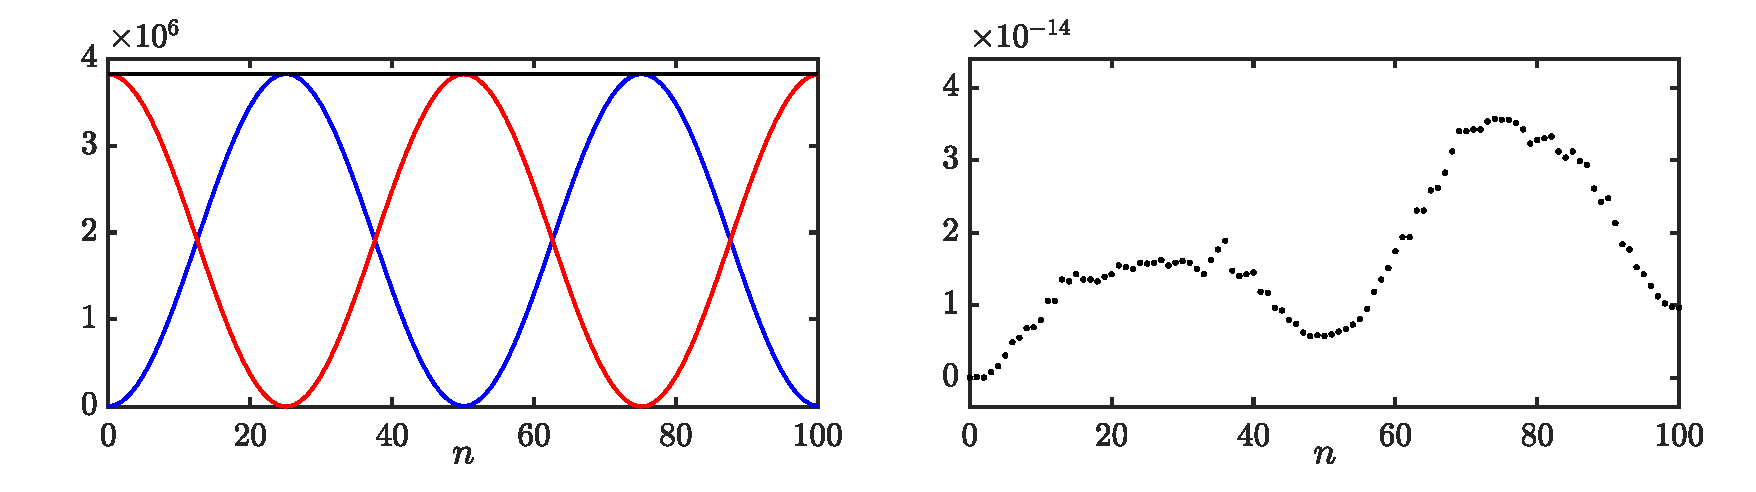
\includegraphics[width=\textwidth]{figures/analysis/massSpringEnergy2.eps}
        };
    
        \node[] (he) at (0.2,0.5) {\small $\mathfrak{h}_\text{e}$};

        \node[] (h) at (-5.75, 1) {\small $\mathfrak{h}$};
        \node[] (v) at (-5.75, 0.5) {\small $\color{red}\mathfrak{v}$};
        \node[] (t) at (-5.75, 0) {\small $\color{blue}\mathfrak{t}$};
      \end{tikzpicture}
      \caption{The kinetic (blue), potential (red), and total (black) energy of an implementation of the mass-spring system are plotted in the left panel. The right panel shows the normalised energy (according to Eq. \eqref{eq:normalisedEnergy}). Notice that the scaling of the y-axis is $10^{-14}$ and the energy is thus within machine precision. \label{fig:energyMassSpring}}
\end{figure}

\subsection{1D wave equation}\label{sec:1DWaveEnergyAnalysis}
Energy analysis could be directly performed on the FD scheme in \eqref{eq:1DwaveFDS}. However, in order for the units of the scheme to add up to energy in Joules, it is useful to write out all physical parameters. Taking the definition for the wave speed for the ideal string $c = \sqrt{T/\rho A}$ and multiplying both sides of Eq. \eqref{eq:1DwaveFDS} by $\rho A$ yields
\begin{equation}\label{eq:1DWavePhysical}
    \rho A \dtt \uln = T \dxx \uln,
\end{equation}
where $l\in d$ with discrete domain $d\in\{0, \hdots, N\}$ and number of grid points $N+1$. Furthermore, Dirichlet boundary conditions as given in Eq. \eqref{eq:discreteDirichlet} are used. A note on using Neumann boundary conditions is given at the end of this section.

\subsubsection{Step 1: Obtain $\dtp \h$}
Taking an inner product using Eq. \eqref{eq:1DWavePhysical} with $\left( \dtd \uln \right)$ and moving all terms to the left-hand side yields the definition for the rate of change of the Hamiltonian:
\begin{equation}\label{eq:rOC1DWave}
    \dtp \h = \rho A \langle \dtd \uln, \dtt \uln \rangle_d - T \langle \dtd\uln, \dxx \uln\rangle_d = 0.
\end{equation}


\subsubsection{Step 2: Identify energy types and isolate $\dtp$}
As in the case of the mass-spring system in the previous section, there are no losses or externally supplied energy present in the system, and all terms are part of the Hamiltonian $\h$.

To isolate $\dtp$ in Eq. \eqref{eq:rOC1DWave}, the terms have to be rewritten in a way that it fits the product identities in Section \ref{sec:prodIdentities}.
Summation by parts as described in Section \ref{sec:summationByParts}  can be used. Using identity \eqref{eq:summationByPartsMinusBar}  with $f_l^n \triangleq \dtd \uln$ and $g_l^n \triangleq \dxp \uln$, the second term can be rewritten to 
%
\begin{equation*}
    - T \langle \dtd\uln, \dxx \uln\rangle_d  = T\langle \dxp(\dtd\uln), \dxp\uln\rangle_{\underline{d}} - \mathfrak{b},
\end{equation*}
where the boundary term
\begin{equation*}
    \mathfrak{b} = T(\dtd u_N^n)(\dxp u_N^n) - T(\dtd u_0^n) \underbrace{(\dxp u_{-1}^n)}_{\dxm u_0^n},
\end{equation*}
and reduced domain $\underline{d} = \{0, \hdots, N-1\}$. As Dirichlet boundary conditions are used, the boundary term vanishes as 
\begin{equation*}
    u_0^n = u_N^n = 0 \quad \Longrightarrow \quad \dtd u_0^n = \dtd u_N^n = 0.
\end{equation*}
In other words, if the states of the system at the boundaries are zero, their velocity will also be zero. 
Then, using the discrete inner product in Eq. \eqref{eq:discInnerProd}, Eq. \eqref{eq:rOC1DWave} can be expanded to
\begin{equation}
    \dtp \h = \rho A \sum_{l = 0}^N h(\dtd \uln)(\dtt \uln) + T \sum_{l = 0}^N h(\dtd \dxp \uln)(\dxp \uln)
\end{equation}
Then, using identities \eqref{eq:prodIdentity1} and \eqref{eq:prodIdentity2}, $\dtp$ can be isolated 
\begin{equation}
    \dtp \h = \dtp \left(\frac{\rho A}{2}\lVert\dtm \uln\rVert^2_d + \frac{T}{2}\langle\dxp\uln, e_{t-}\dxp\uln\rangle_{\underline{d}}\right),
\end{equation}
and the definition for the Hamiltonian and the kinetic and potential energy can be found:
\begin{equation}\label{eq:energyBalance1DWave}
    \begin{gathered}
        \h = \t + \v,\\
        \text{with}\quad \t = \frac{\rho A}{2}\lVert\dtm \uln\rVert^2_d, \qaq \v = \frac{T}{2}\langle\dxp\uln, e_{t-}\dxp\uln\rangle_{\underline{d}}.
    \end{gathered}
\end{equation}

\subsubsection{Step 3: Check units}
Writing out the definitions for kinetic and potential energy in Eq. \eqref{eq:energyBalance1DWave} respectively, yields
\begin{align*}
    \t = \frac{\rho A}{2}\lVert\dtm \uln\rVert^2_d \overset{\text{in units}}{\xrightarrow{\hspace*{1cm}}}& \ \text{kg}\cdot \text{m}^{-3} \cdot \text{m}^2\cdot \text{m} \cdot(\text{s}^{-1}\cdot \text{m})^{2}\\
    & = \text{kg}\cdot\text{m}^2\cdot\text{s}^{-2},\\
    \v = \frac{T}{2}\langle\dxp\uln, e_{t-}\dxp\uln\rangle_{\underline{d}}\overset{\text{in units}}{\xrightarrow{\hspace*{1cm}}}& \ \text{N} \cdot \text{m}\cdot (\text{m}^{-1}\cdot\text{m}\cdot \text{m}^{-1}\cdot\text{m}^{-1}\text{m}) \\
    & = \text{kg} \cdot \text{m}^2 \cdot \text{s}^{-2},
\end{align*}
and are indeed in Joules. Notice that an extra `m' unit appears due to the norm and inner product.

\subsubsection{Step 4: Implementation}
The energy balance in Eq. \eqref{eq:energyBalance1DWave} can be implemented with the following code in the for-loop recursion:

\setlstMAT
\begin{lstlisting}
%% Calculate the energy using Eq. %*\eqrefMatlab[eq:energyBalance1DWave]*) 

% Kinetic energy
kinEnergy(n) = rho * A / 2 * h * sum((1/k * (u-uPrev)).^2);

% Potential energy
potEnergy(n) = T/(2*h) * sum(([u; 0] - [0; u]) ...
            .* ([uPrev; 0] - [0; uPrev]));

% Total energy (Hamiltonian)
totEnergy(n) = kinEnergy(n) + potEnergy(n);
\end{lstlisting}
Here, \texttt{u} is the vector $\u = [u_1^n, \hdots, u_{N-1}^n]^T$ (as Dirichlet boundary conditions are used) and need to be concatenated with $0$ in the calculation of the potential energy as the boundaries needs to be included in the calculation, despite them being 0!\footnote{As can be seen from the definition of $\v$ in Eq. \eqref{eq:energyBalance1DWave}, the domain used for the inner product is $\underline{d} = \{0,\hdots, N-1\}$ and $\v$ contains a forward difference in its definition requiring $u_N^n$ as well.}
Figure \ref{fig:energy1DWave} shows the plot of the normalised energy according to Eq. \eqref{eq:normalisedEnergy} and shows that the deviation of $\h^n$ is within machine precision.
\begin{figure}[h]
    \centering
    \begin{tikzpicture}[->,node distance=3cm,
        thick,main node/.style={circle,draw}]
    
        \node[] (image) at (0,0) {
        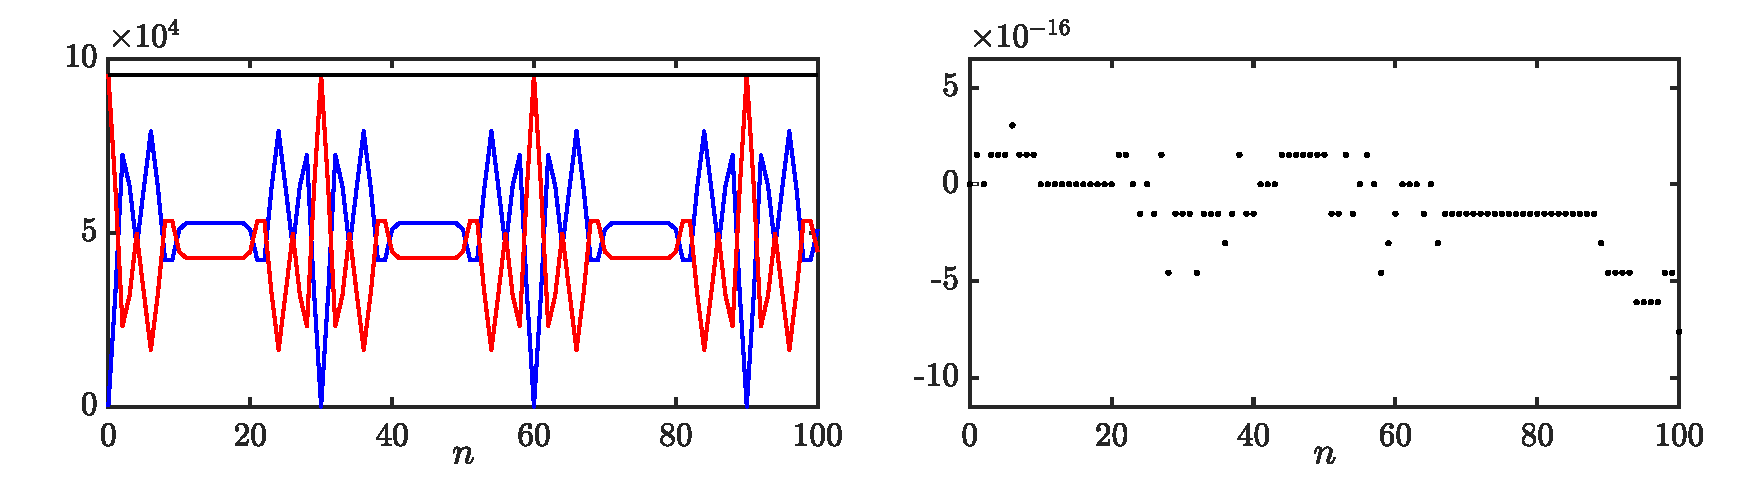
\includegraphics[width=\textwidth]{figures/analysis/1dWaveEnergy.eps}
        };
    
        \node[] (he) at (0.2,0.5) {\small $\mathfrak{h}_\text{e}$};

        \node[] (h) at (-5.75, 1) {\small $\mathfrak{h}$};
        \node[] (v) at (-5.75, 0.5) {\small $\color{red}\mathfrak{v}$};
        \node[] (t) at (-5.75, 0) {\small $\color{blue}\mathfrak{t}$};
      \end{tikzpicture}
      \caption{The kinetic (blue), potential (red), and total (black) energy of an implementation of the 1D wave equation are plotted in the left panel. The right panel shows the normalised energy (according to Eq. \eqref{eq:normalisedEnergy}) and shows that the deviation of the energy is within machine precision. \label{fig:energy1DWave}}
\end{figure}

\subsubsection{Neumann boundary conditions}
If Neumann boundary conditions -- as per Eq. \eqref{eq:discreteNeumann} -- are used instead, the primed inner product in Eq. \eqref{eq:primedInnerProd} needs to be used in Step 1. Using the identity in \eqref{eq:primedIdentityMinus}, summation by parts of the second term results in
\begin{equation*}
    - T \langle \dtd\uln, \dxx \uln\rangle_d'  = T\langle \dxp(\dtd\uln), \dxp\uln\rangle_{\underline{d}} - \mathfrak{b},
\end{equation*}
where the boundary term
\begin{align*}
    \mathfrak{b} &= T(\dtd u_N^n)(\mxm\dxp u_N^n) - T(\dtd u_0^n) (\mxm \dxp u_0^n),\\[-1em]
    \xLeftrightarrow{\mystrut\ \text{Eq. \eqref{eq:identity2}}\ } \quad &= T(\dtd u_N^n)(\dxd u_N^n) - T(\dtd u_0^n) (\dxd u_0^n).
\end{align*}
As the Neumann boundary condition states that
\begin{equation*}
    \dxd u_0^n = \dxd u_N^n = 0
\end{equation*}
the boundary term vanishes and the energy balance results in
%
\begin{equation}\label{eq:energyBalance1DWaveNeumann}
    \begin{gathered}
        \h = \t + \v,\\
        \text{with}\quad \t = \frac{\rho A}{2}\Big(\lVert \dtm \uln \rVert'_d\Big)^2, \qaq \frac{T}{2}\langle\dxp\uln, e_{t-}\dxp\uln\rangle_{\underline{d}}.
    \end{gathered}
\end{equation}
Using \texttt{u} for the vector $\u = [u_0^n, \hdots, u_N^n]^T$, this is then implemented as

\setlstMAT
\begin{lstlisting}
%% Calculate the energy using Eq. %*\eqrefMatlab[eq:energyBalance1DWaveNeumann]*) 

% Scaling of the boundaries through weighted inner product
scaling = [0.5; ones(N-1, 1); 0.5];

% Kinetic energy
kinEnergy(n) = rho * A / 2 * h * sum(scaling .* (1/k * (u-uPrev)).^2);

% Potential energy
potEnergy(n) = T/(2*h) * sum(u(2:end) - u(1:end-1) ...
            .* (uPrev(2:end) - uPrev(1:end-1)));

% Total energy (Hamiltonian)
totEnergy(n) = kinEnergy(n) + potEnergy(n);
\end{lstlisting}


\subsection{Stability using energy analysis techniques}\label{sec:stabilityAnalysisEnergy}
Section \ref{sec:stabilityAnalysis} showed how to obtain a stability condition of a FD scheme using a frequency domain representation. Although not operating in the frequency domain, the energy analysis techniques presented here may also be used to obtain stability conditions of FD schemes and might even be considered more powerful than the frequency domain approach, as it can also be used to analyse spatially varying and nonlinear systems!\todo{long sentence}

To arrive at a stability condition, the energy must be \textit{non-negative} ($\h \geq 0$) or, in some cases \textit{positive definite} ($\h > 0$). Below, the mass-spring system and the 1D wave equation will be used as a test case.

\subsubsection{Mass-spring system}
Section \ref{sec:massSpringStability} mentions that the mass-spring system is a special case in that the roots of its characteristic equation can not be identical. When proving stability using energy analysis, this means that the energy of the system needs to be positive definite. It can be shown that an equation of the form 
\begin{equation}\label{eq:quadraticForm}
    x^2 + y^2  + 2axy
\end{equation} 
is positive definite if $|a| < 1$.% If $|a| = 1$, the function is non-negative, but not positive definite.

Equation \eqref{eq:quadraticForm} can be used to prove stability for the mass spring system using the energy balance in Eq. \eqref{eq:energyBalanceMassSpring}. One can easily conclude that $\t$ is non-negative due to the fact that  $M > 0$ and $(\dtm \un)$ is squared. The potential energy $\v$, however, is of indefinite sign. Expanding the operators in Eq. \eqref{eq:energyBalanceMassSpring} yields
\begin{align*}
    \h &= \frac{M}{2k^2}\Big((\un)^2 - 2\un u^{n-1} + (u^{n-1})^2\Big)+ \frac{K}{2}\un u^{n-1},\\
    &= \frac{M}{2k^2}\Big((\un)^2+ (u^{n-1})^2\Big)+ \left(\frac{K}{2}-\frac{M}{k^2}\right)\un u^{n-1}.
\end{align*}
Dividing all terms by $M/2k^2$ this equation is of the form in Eq. \eqref{eq:quadraticForm}:
\begin{equation*}
    \h = (\un)^2+ (u^{n-1})^2+ \left(\frac{Kk^2}{M} - 2\right)\un u^{n-1}.
\end{equation*}
For $\h$ to be positive definite, the following condition must hold
\begin{equation*}
    \left|\frac{Kk^2}{2M} - 1\right| < 1.
\end{equation*}
This can then be written as
\begin{align*}
    -1&<\frac{Kk^2}{2M} - 1<1\\
    0 &< \frac{Kk^2}{2M} < 2
\end{align*}
where, as long as $K$ and $k$ are non-zero, the first inequality is always satisfied. Then the condition solved for $k$ can easily be shown to be
\begin{equation}
    k < 2\sqrt{\frac{M}{K}}
\end{equation}
which is identical to the definition in Eq. \eqref{eq:stabilityMK}.

\subsubsection{1D wave equation}
For the 1D wave equation, the energy must be proven to be non-negative. One can take the energy balance in Eq. \eqref{eq:energyBalance1DWave} and conclude that $\t$ is non-negative due to the non-negativity of the parameters and $(\dtm \uln)$ being squared. The potential energy, however, is of indefinite sign. One can rewrite $\v$ using identity \eqref{eq:prodIdentityEnergyStab} as
\begin{align*}
    \v &= \frac{T}{2} \langle \dxp \uln, e_{t-}\dxp \uln\rangle_{\underline{d}},\\
    &= \frac{T}{2} \sum_{l=0}^{N-1} h(\dxp \uln)(e_{t-}\dxp\uln),\\
    &= \frac{T}{2} \sum_{l=0}^{N-1} h\left((\mtm \dxp \uln)^2 - \frac{k^2}{4}(\dtm\dxp \uln)^2\right),\\
    &= \frac{T}{2}\left(\lVert\mtm\dxp\uln\rVert_{\underline{d}}^2-\frac{k^2}{4}\lVert\dtm\dxp \uln\rVert_{\underline{d}}^2\right).
\end{align*}
One can then use the following bound for spatial differences \cite{theBible}
\begin{equation}\label{eq:spatialBound}
    \lVert \dxp \uln \rVert_{\underline{d}} \leq \frac{2}{h}\lVert \uln \rVert_d' \leq \frac{2}{h}\lVert \uln \rVert_d,
\end{equation}
to put a condition on $\v$
\begin{align*}
    \v &\geq \frac{T}{2}\left(\lVert\mtm\dxp\uln\rVert_{\underline{d}}^2 - \frac{k^2}{4}\left(\frac{2}{h}\lVert\dtm\uln\rVert_{d}\right)^2\right),\\
    &\geq \frac{T}{2}\left(\lVert\mtm\dxp\uln\rVert_{\underline{d}}^2 - \frac{k^2}{h^2}\lVert\dtm\uln\rVert_{d}^2\right),
\end{align*}
Substituting this condition into the energy balance in Eq. \eqref{eq:energyBalance1DWave} yields
\begin{align*}
    \h = \t + \v &\geq \frac{\rho A}{2}\lVert\dtm \uln\rVert^2_d + \frac{T}{2}\left(\lVert\mtm\dxp\uln\rVert_{\underline{d}}^2 - \frac{k^2}{h^2}\lVert\dtm\uln\rVert_{d}^2\right),\\
    &\geq \left(\frac{\rho A}{2} - \frac{Tk^2}{2h^2}\right)\lVert \dtm \uln\rVert_d^2 + \frac{T}{2}
    \lVert\mtm\dxp \uln\rVert_{\underline{d}}^2.
\end{align*}
Recalling that $c = \sqrt{T /\rho A}$ and $\lambda = ck/h$, all terms can be divided by $\rho A$ which yields
\begin{equation}
    \h = \t + \v \geq \frac{1}{2}\left(1 - \lambda^2\right)\lVert \dtm \uln\rVert_d^2 + \frac{c^2}{2}
    \lVert\mtm\dxp \uln\rVert_{\underline{d}}^2,
\end{equation}
and is non-negative for
\begin{align*}
    1-\lambda^2 &\geq 0,\\
    \lambda &\leq 1.
\end{align*}
This is the same (CFL) condition obtained through von Neumann analysis in Section \ref{sec:vonNeumann1DWave}.

\section{Modal analysis}
\label{sec:modalAnalysis}
Modes are the resonant frequencies of a system. The number of modes that a discrete system contains depends on the number of moving points. A mass-spring system thus has one resonating mode, but -- as briefly touched upon in Section \ref{sec:output1DWave} -- a FD scheme of the 1D wave equation with $N = 30$ and Dirichlet boundary conditions will have $29$ modes. Modal analysis \todo{some citation here} can be used to obtain objective data on what modes a FD scheme should contain. This can then be used to determine whether this matches one's expectations or whether the output of the system matches what the analysis predicted. This section will show how to numerically obtain the modal frequencies of a FD implementation using the 1D wave equation as a test case.

Recall the matrix form of the 1D wave equation from Eq. \eqref{eq:1DwaveMatrix}
\begin{equation*}
    \frac{1}{k^2}\left(\u^{n+1}-2\u^n+\u^{n-1}\right) = c^2 \Dxx\u^n.
\end{equation*}
Following \cite{theBible}, a test solution of the form $\u^n = z^n\boldPhi$ can be assumed \todo{more explanation, perhaps refer to von neumann analysis in \ref{sec:stabilityAnalysis}}. Substituting this into the above equation yields the characteristic equation
\begin{equation}
    (z - 2 + z^{-1})\boldPhi = c^2k^2\Dxx \boldPhi.
\end{equation}
This is an eigenvalue problem (see Section \ref{sec:eigenValueProblems}) where the $p$\th solution $\boldPhi_p$ may be interpreted as the modal shape of mode $p$. The corresponding modal frequencies are the solutions to the following equations:
\begin{gather}\label{eq:1DWaveModalIntermediate}
    z_p-2+z_p^{-1} = c^2k^2\text{eig}_p(\Dxx),\nonumber\\
    z_p+\Big(-2-c^2k^2\text{eig}_p(\Dxx)\Big)+z_p^{-1}=0.
\end{gather}
%\SWcomment[If the CFL condition for the scheme is satisfied, the roots will lie on the unit circle.] 
Furthermore, one can substitute a test solution $z_p = e^{s_pk}$ with complex frequency $s_p = j\omega_p + \sigma_p$ which contains the (angular) frequency $\omega_p$ and damping $\sigma_p \leq 0$ \todo{check with Stefan} of the $p$\th mode.\footnote{Notice that regardless of the possible damping coefficient per mode, the eventual amplitude of each will mostly be determined by the locations of the excitation and output as discussed in Section \ref{sec:output1DWave}.} As there is no damping present in the system, the test solution reduces to $z_p = e^{j\omega_p k}$ which can be substituted into Eq \eqref{eq:1DWaveModalIntermediate} to get
\begin{align*}
    e^{j\omega_pk}+e^{-j\omega_pk}-2-c^2k^2\text{eig}_p(\Dxx)&=0,\\
    \frac{e^{j\omega_pk}+e^{-j\omega_pk}}{-4}+\frac{1}{2}+\frac{c^2k^2}{4}\text{eig}_p(\Dxx)&=0.
\end{align*}
Finally, using the trigonometric identity in Eq. \eqref{eq:sinIdentity} yields
\begin{align}
    \sin^2(\omega_pk/2)&+\frac{c^2k^2}{4}\text{eig}_p(\Dxx)=0,\nonumber\\
    \sin(\omega_pk/2)&=\frac{ck}{2}\sqrt{-\text{eig}_p(\Dxx)},\nonumber\\
    \omega_p &= \frac{2}{k}\sin^{-1}\left(\frac{ck}{2}\sqrt{-\text{eig}_p(\Dxx)}\right),\label{eq:1DWaveModesAngular}
\end{align}
and can be rewritten to 
\begin{equation}
    f_p = \frac{1}{\pi k}\sin^{-1}\left(\frac{ck}{2}\sqrt{-\text{eig}_p(\Dxx)}\right)\label{eq:1DWaveModes}
\end{equation}
to get the modal frequency of the $p$\th mode in Hz. 

See Figure \ref{fig:modalFreqs1Dwave} for a plot of the modal frequencies of an implementation of the 1D wave equation with the parameters given in Table \ref{tab:1DWaveParams}.
The figure shows one great advantage of performing modal analysis on an FD scheme, over only obtaining the spectrum of its output. Although the values from the analysis do correspond to the partials shown in the frequency domain output of the 1D wave equation in Figure \ref{fig:1DWaveOutput}, the latter does not show all modes present in the system. This is due to the input and output locations of the system as discussed in Section \ref{sec:output1DWave}. The modal analysis does obtain the frequency data regardless of the aforementioned input and output locations. 

\begin{figure}[h]
    \centering
    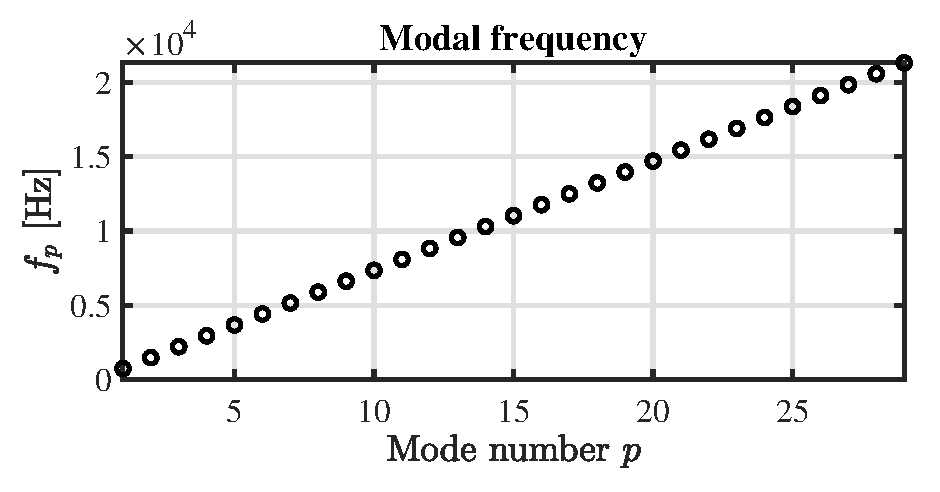
\includegraphics[width = 0.6\textwidth]{figures/analysis/1dmodes.eps}
    \caption{Modal frequencies of the 1D wave equation with the parameters given in Table \ref{tab:1DWaveParams}. \label{fig:modalFreqs1Dwave}}
\end{figure}

\subsection{One-step form}\label{sec:oneStepForm}
For more complicated systems, specifically those containing damping terms, it is useful to rewrite the update in \textit{one-step form} (also referred to as a state-space representation). The damping terms cause the coefficients of $z$ and $z^{-1}$ in the characteristic equation to not be identical and the trigonometric identities in \eqref{eq:trigIdentities} can not be used directly. Although the eigenfrequency calculation needs to be done on a larger matrix, it allows for a more general and direct way to calculate the modal frequencies and damping coefficients per mode. 

If matrix $\A$ has an inverse, any scheme of the form
\begin{equation}\label{eq:modalForm}
    \A\u^{n+1}=\B\u^n + \C\u^{n-1},
\end{equation}
can be rewritten to
\begin{equation}\label{eq:oneStepForm}
    \underbrace{\begin{bmatrix}
        \u^{n+1}\\
        \u^n
    \end{bmatrix}}_{\w^{n+1}} = 
    \underbrace{\begin{bmatrix}
        \A^{-1}\B & \A^{-1}\C\\
        \I & \mathbf{0}
    \end{bmatrix}}_{\Q}
    \underbrace{\begin{bmatrix}
        \u^n\\
        \u^{n-1}
    \end{bmatrix}}_{\w^n}
\end{equation}
which relates the unknown state of the system to the known state through matrix $\Q$ which encompasses the scheme. The sizes of the identity matrix $\I$ and zero matrix $\mathbf{0}$ are the same size as $\A, \B$ and $\C$.

Again, solutions of the form $\w^n = z^n\boldPhi$ can be assumed (where $\boldPhi$ is now less-trivially connected to the modal shapes)
\begin{equation}
    z\boldPhi = \Q\boldPhi ,
\end{equation}
which can be solved for the $p$th eigenvalue as
\begin{equation}
    z_p = \text{eig}_p(\Q).
\end{equation}
As the scheme could exhibit damping, the test solution $z_p = e^{s_pk}$ is used. Substituting this yields
\begin{align}
    e^{s_pk} &= \text{eig}_p(\Q),\nonumber\\
    s_p &= \frac{1}{k}\ln \left(\text{eig}_p(\Q)\right).\label{eq:sp}
\end{align}
Solutions for the frequency and damping for the $p$th eigenvalue can then be obtained through
\begin{equation}
    \omega_p = \mathfrak{I}(s_p) \quad \text{and} \quad \sigma_p = \mathfrak{R}(s_p),
\end{equation}
where $\mathfrak{I}(\cdot)$ and $\mathfrak{R}(\cdot)$ denote the ``imaginary part of'' and ``real part of'' respectively. 

As the elements of $\Q$ are real-valued, the solutions $s_p$ in Eq. \eqref{eq:sp} come in complex conjugates (pairs of numbers of which the imaginary part has an opposite sign). For analysis, only the $\mathfrak{I}(s_p)\geq 0$ should be considered as these correspond to non-negative frequencies. 

\section{Conclusion}
This chapter presented three different analysis techniques in discrete time, that are of extreme utility when working with FD schemes. Frequency domain analysis, or von Neumann analysis in the distributed case, can be used to obtain stability conditions for LTI and LSI systems. Energy analysis techniques can also be used to prove stability and passivity, but for a larger range of systems including LTI, LSI, and nonlinear systems. Furthermore, energy analysis can be used in a practical manner to debug implementations of FD schemes and ensure that no programming errors have been made. Finally, modal analysis can be used to analyse the behaviour of a scheme in terms of its modal frequencies and modal shapes. This can be used to determine whether the auditory output matches the precidictions of the analysis. Although analogous techniques in continuous time also exist, a more practical angle has been chosen for this work and only the discrete time methods have been presented. For more information about the techniques in continuous time, see \cite{theBible}.

All three analysis techniques will be extensively used in the rest of this document to analyse the FD schemes used in this project.